% Source: Weinberg GR, physical PDF p. 593 (printed p. 565).
% Coverage: Figure 15.6, Jeans mass versus radiation temperature.
% Status: source-reviewed and compile-clean; visually proofed.
% Uncertainties: none.

\begingroup
\renewcommand{\thefigure}{15.6}
\begin{figure}[htbp]
  \centering
  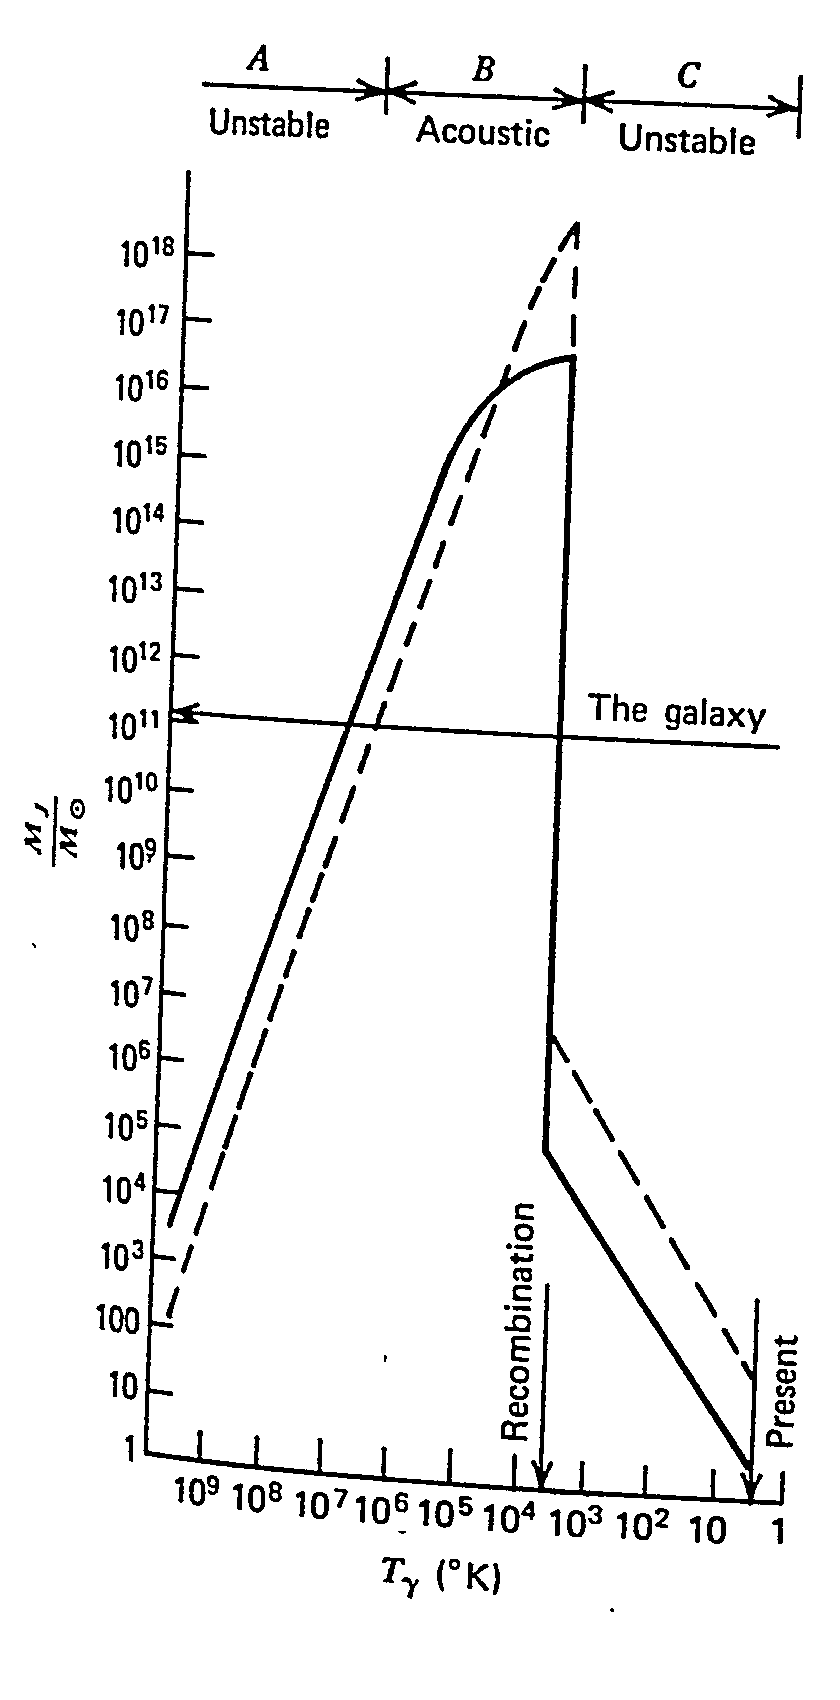
\includegraphics[height=0.68\textheight]{figures/chapter15/fig15-06.png}
  \caption{Jeans mass as a function of radiation temperature. Solid line is
  for \(\sigma=0.8\times10^8\), corresponding to
  \(T_{\gamma0}=2.7^\circ\mathrm K\),
  \(\rho_0=3\times10^{-29}\,\mathrm{g/cm^3}\). Dashed line is for
  \(\sigma=2.4\times10^9\), corresponding to
  \(T_{\gamma0}=2.7^\circ\mathrm K\),
  \(\rho_0=10^{-30}\,\mathrm{g/cm^3}\). The drop in Jeans mass at
  recombination is somewhat more gradual than shown here.}
  \label{fig:15.6}
\end{figure}
\endgroup
